
The class \verb+Polyhedron_3+ can represent polygon
meshes\footnote{\href{http://www.cgal.org/Manual/doc_html/basic_lib/Polyhedron_ref/Class_Polyhedron_3.html}{http://www.cgal.org}}.
Its underlying combinatorial component is based on the halfedge data
structure. As all CGAL geometric entities, its geometric component is
templated by the
\italic{kernel}\footnote{\href{http://www.CGAL.org/Manual/doc_html/frameset/fsKernel.html}{CGAL kernel}}.

\subsubsection{Declaration}

The simplest declaration of the polyhedron (without extended
primitives) consists of templating with a cartesian kernel and double
number precision:

{ \scriptsize
\begin{verbatim}
// instanciation of a polyhedron

#include <CGAL/Cartesian.h>
#include <CGAL/Polyhedron_3.h>

typedef CGAL::Cartesian<double>     kernel;
typedef CGAL::Polyhedron_3<kernel>  Polyhedron;

Polyhedron p;
\end{verbatim}}

\subsubsection{Extending primitives}

The polyhedron can be parameterized by a \italic{traits} class in
order to extend the vertex, halfedge and facet primitives. In this
tutorial all primitives (facets, halfedges and vertices) are
extended. The facet is extended with a normal and with a
general-purpose integer tag:

{ \scriptsize
\begin{verbatim}

template <class	Refs, class T, class P, class Norm>
class Enriched_facet : 
  public CGAL::HalfedgeDS_face_base<Refs, T>
{
  // tag
  int m_tag;

  // normal
  Norm m_normal;

public:

  // no  constructors to  repeat,  since  only
  // default constructor mandatory
  Enriched_facet()
  {
  }

  // tag
  const int&  tag()  {  return m_tag;  }
  void tag(const int& t)  {  m_tag  =  t; }

  // normal
  typedef  Norm Normal_3;
  Normal_3&  normal() { return  m_normal;  }
  const  Normal_3&  normal() const { return  m_normal;  }
};
\end{verbatim}}

The halfedge is extended with a general-purpose tag and a binary tag
to indicate wether it belongs to the control mesh or not. The latter
tag is used to superimpose the control mesh as shown in
Fig.\ref{fig:teaser}.

{ \scriptsize
\begin{verbatim}

template <class  Refs, class Tprev, class Tvertex, 
          class Tface, class Norm>
class Enriched_halfedge : public 
  CGAL::HalfedgeDS_halfedge_base<Refs,Tprev,Tvertex,Tface>
{
private:

  // tag
  int  m_tag; 

  // option  for control edge superimposing
  bool m_control_edge; 

public:

  // life  cycle
  Enriched_halfedge()
  {
    m_control_edge = true;
  }

  // tag
  const int& tag() const { return m_tag;  }
  int& tag() { return m_tag;  }
  void tag(const int& t)  {  m_tag  =  t; }

  // control edge  
  bool& control_edge()  { return m_control_edge; }
  const bool& control_edge()  const { return m_control_edge; }
  void control_edge(const bool& flag) { m_control_edge  =  flag;  }
};

\end{verbatim}}

The vertex is extended with a normal and a general-purpose integer
tag:

{ \scriptsize
\begin{verbatim}


template <class  Refs, class T, class P, class Norm>
class Enriched_vertex :  
  public CGAL::HalfedgeDS_vertex_base<Refs, T, P>
{
  // tag
  int  m_tag; 

  // normal
  Norm m_normal;

public:
  // life  cycle
  Enriched_vertex() {}
  // repeat  mandatory  constructors
  Enriched_vertex(const  P& pt)
    :  CGAL::HalfedgeDS_vertex_base<Refs, T,  P>(pt)
  {
  }

  // normal
  typedef  Norm Normal_3;
  Normal_3&  normal() { return  m_normal;  }
  const  Normal_3&  normal() const { return  m_normal;  }

  // tag
  int& tag() {  return m_tag;  }
  const int& tag() const {  return m_tag;  }
  void tag(const int& t)  {  m_tag  =  t; }
};

\end{verbatim}}



A redefined items class for the polyhedron uses the class wrapper
mechanism to embedd all three extended primitives within one unique
class.

{ \scriptsize
\begin{verbatim}

struct Enriched_items : public CGAL::Polyhedron_items_3
{
    // wrap  vertex
    template <class  Refs,  class  Traits>
    struct Vertex_wrapper
    {
        typedef  typename Traits::Point_3  Point;
        typedef  typename Traits::Vector_3  Normal;
        typedef  Enriched_vertex<Refs,
                          CGAL::Tag_true,
                          Point,
                          Normal>  Vertex;
    };

    // wrap  face
    template <class  Refs,  class  Traits>
    struct Face_wrapper
    {
        typedef  typename Traits::Point_3  Point;
        typedef  typename Traits::Vector_3  Normal;
        typedef  Enriched_facet<Refs,
                         CGAL::Tag_true,
                         Point,
                         Normal> Face;
    };

    // wrap  halfedge
    template <class  Refs,  class  Traits>
    struct Halfedge_wrapper
    {
        typedef  typename Traits::Vector_3  Normal;
        typedef  Enriched_halfedge<Refs,
                            CGAL::Tag_true,
                            CGAL::Tag_true,
                            CGAL::Tag_true,
                            Normal>  Halfedge;
    };
};
\end{verbatim}}

The trait class is then used for templating a polyhedron
\italic{Enriched\_polyhedron}:

{ \scriptsize
\begin{verbatim}

template <class  kernel,  class  items>
class  Enriched_polyhedron :
  public CGAL::Polyhedron_3<kernel,items>
{
  //...
};
\end{verbatim}}

The corresponding instanciation of an enriched polyhedron follows:

{ \scriptsize
\begin{verbatim}

#include <CGAL/Simple_cartesian.h>
#include "enriched_polyhedron.h"

typedef double number_type;
typedef CGAL::Simple_cartesian<number_type> kernel;

Enriched_polyhedron<kernel,Enriched_items> polyhedron;

\end{verbatim}}


\subsubsection{Iteration and Circulation}

The \italic{iterator} STL concept allows traversing a sequence of
items. This concept is applied to the primitives of a mesh, be they
halfedges, edges, vertices, facets or points. Notice that the order of
iteration is not dictated by any incidence relationship, contrary to
the circulator. The following example shows how to iterate on the mesh
vertices.

{ \scriptsize
\begin{verbatim}
Vertex_iterator iter;
for(iter = polyhedron.vertices_begin();
    iter != polyhedron.vertices_end();
    iter++)
{
  Vertex_handle hVertex = iter;
  // do something with hVertex
}
\end{verbatim}}

The \italic{circulator} STL concept allows traversing a circular
sequence of items. This concept is applied both inside facets and
around vertices. 

\paragraph{Circulating around a facet}
The facets being defined by the circular sequence of halfedges along
their boundary, this calls for a circulator around a facet. The
convention is that the halfedges are oriented counterclockwise around
facets as seen from the outside of the polyhedron (see
Fig.\ref{fig:stl_concept}, left).

{ \scriptsize
\begin{verbatim}
// circulate around hFacet
Halfedge_around_facet_circulator circ = hFacet->facet_begin();
Halfedge_around_facet_circulator end = circ;
CGAL_For_all(circ,end)
{
  Halfedge_handle hHalfedge = circ;
  // do something with hHalfedge
}
\end{verbatim}}

\paragraph{Circulating around a vertex}
The convention being that the halfedges are oriented counterclockwise
around facets as seen from the outside of the polyhedron, this implies
that the halfedges are oriented clockwise around the vertices (see
Fig.\ref{fig:stl_concept}, right).

{ \scriptsize
\begin{verbatim}
// circulate around hVertex
Halfedge_around_vertex_circulator circ = hVertex->vertex_begin();
Halfedge_around_vertex_circulator end = circ;
CGAL_For_all(circ,end)
{
  Halfedge_handle hHalfedge = circ;
  // do something with hHalfedge
}
\end{verbatim}}

% circulation inside a facet and around a vertex
\begin{figure}[htb]
    \centering{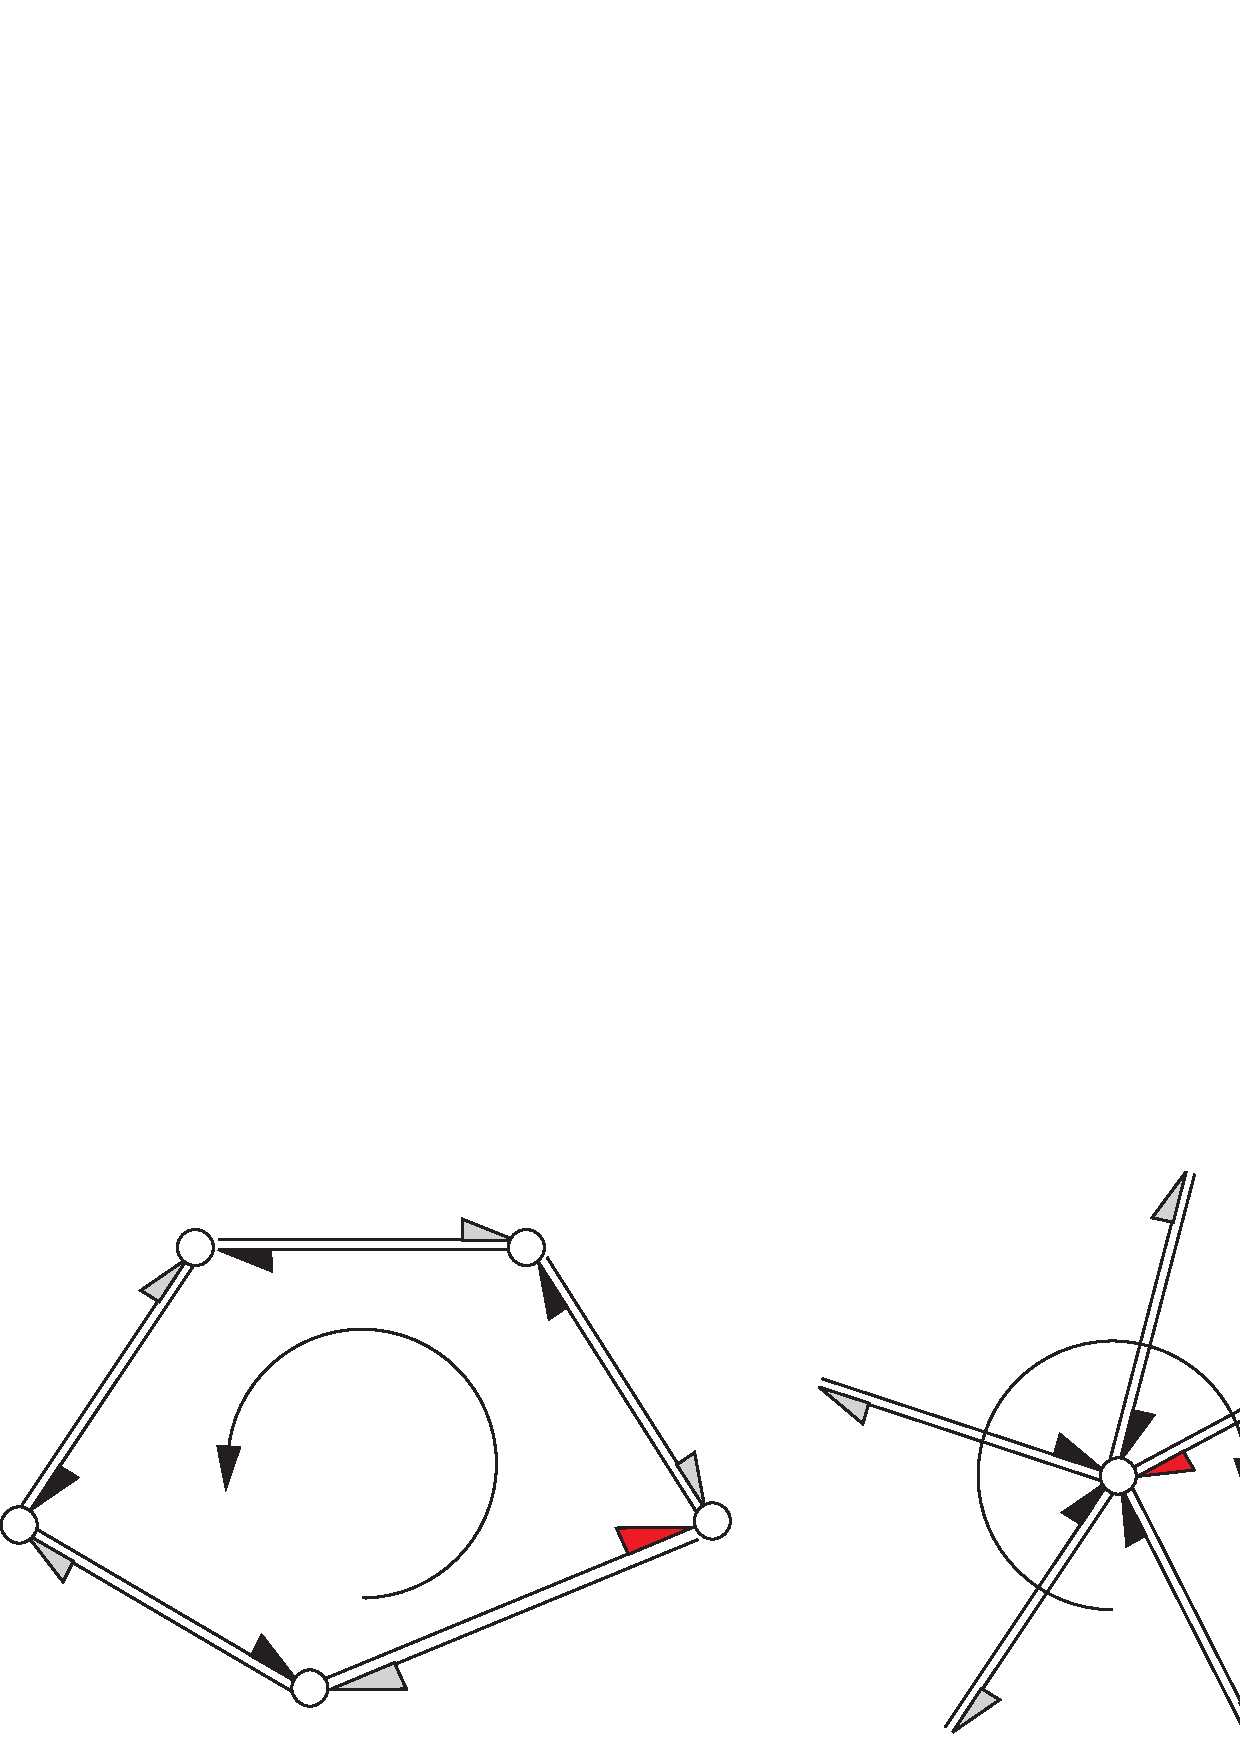
\includegraphics[width=7.0cm]{figs/stl_concepts}}
    \caption{Left: circulation around a facet (ccw).
             Right: circulation around a vertex (cw).}  
    \label{fig:stl_concept}
\end{figure}
